\documentclass[10pt,letterpaper,twocolumn]{article}
\usepackage[letterpaper,top=.72in,bottom=.72in,left=.68in,right=.68in,columnsep=.25in]{geometry}
\usepackage{fontspec}
\setmainfont{lmroman10-regular.otf}[BoldFont=lmroman10-bold.otf,ItalicFont=lmroman10-italic.otf,BoldItalicFont=lmroman10-bolditalic.otf]
\setsansfont{lmsans10-regular.otf}[BoldFont=lmsans10-bold.otf]
\usepackage{amsmath,amssymb,graphicx,microtype}
\usepackage[font=small,labelfont=bf]{caption}
\usepackage[hidelinks]{hyperref}
\usepackage{xcolor}
\definecolor{linktone}{HTML}{245C55}
\hypersetup{colorlinks=true,linkcolor=linktone,citecolor=linktone,urlcolor=linktone,
pdftitle={The Developmental Regulatory Cascade},pdfauthor={E. T. Ellis}}
\setlength{\parindent}{1em}
\setlength{\parskip}{0pt}
\emergencystretch=1em
\raggedbottom
\begin{document}
\twocolumn[{
\begin{center}
{\small\sffamily\bfseries RESEARCH ARTICLE}\\[.7em]
{\huge\bfseries The Developmental Regulatory Cascade}\\[.6em]
{\large Constitution, perinatal initialization, and the \ensuremath{\alpha_2\delta}--CaV2 hinge in a coupled organism--environment research program}\\[1em]
{\normalsize E. T. Ellis}\\
{\small Independent researcher \quad \textbullet \quad 25 September 2026}\\[.45em]
{\small Working hypothesis manuscript v1.1 \quad \textbullet \quad Not peer reviewed}
\end{center}
\vspace{.25em}
\begin{center}
\begin{minipage}{.86\textwidth}
\begin{center}\normalsize\sffamily\bfseries Abstract\end{center}
\vspace{.1em}
\small Heterogeneous developmental phenotypes are poorly represented by a single line from a gene or exposure to a diagnosis. This article synthesizes the RCCX–Hunter–Dąbrowski Cascade, the Perinatal Regulatory Initialization extension, and the organism–environment interface of The Polymathic Singularity into a modular causal research program. We propose that constitutional variation interacts with perinatal endocrine, microbial, immune, sensory, and affiliative conditions to influence developing regulation. The \ensuremath{\alpha_2\delta}–CaV2 system is examined as a candidate convergence mechanism because experimentally established roles in channel trafficking, presynaptic release, and thrombospondin-dependent synaptogenesis create several possible routes from developmental conditions to network organization. The crucial connection from ordinary perinatal variation to this molecular system remains unproven. Maternal microbial inheritance and the Limosilactobacillus reuteri–vagal–oxytocin pathway supply complementary, partly independent hypotheses; mouse mechanisms and preliminary human interventions are kept distinct. Regulatory Closure Bias is formalized as a proposed, context-dependent contrast between gains obtained through external interaction and internally sustained stabilization. Hunter/Farmer and Dąbrowski terminology are retained as ecological and developmental interpretations rather than genetic categories or validated biological stages. Time-indexed causal graphs preserve feedback without introducing cycles into a single-time causal DAG. An evidence ledger separates demonstrated mechanisms, supported syntheses, proposed bridges, and horizon hypotheses. Three core studies target the molecular bridge, longitudinal mediation, and phenotype–environment interaction; a contingent intervention study follows only if these justify it. The framework is intended to organize discriminating experiments, not establish a unitary cause of autism, infer developmental lesions from adult drug responses, or rank human phenotypes.

\vspace{.55em}
\noindent\textbf{Keywords:} neurodevelopment; perinatal regulation; CACNA1B; CACNA2D; \ensuremath{\alpha_2\delta}; microbiome; regulatory coupling; causal inference; developmental heterogeneity; human–AI interaction
\end{minipage}
\end{center}
\vspace{1em}
}]
\section{Introduction}

A developmental phenotype is a trajectory through interacting constraints. Genes, tissue mechanics, endocrine signaling, immune activity, experience, and available environments can affect one another over time. A diagnosis may summarize recurring outcomes without identifying the particular sequence that produced them. The practical challenge is to describe this coupling without converting every plausible association into a causal explanation.

The present synthesis makes one organizing proposal: constitutional variation and early regulatory conditions may converge partly through synaptic developmental machinery, altering the conditions under which sensory processing, autonomic regulation, attention, affiliation, and action become coordinated. The central sequence is Constitution \ensuremath{\rightarrow} Perinatal Initialization \ensuremath{\rightarrow} \ensuremath{\alpha_2\delta}–CaV2 Hinge \ensuremath{\rightarrow} Network Calibration \ensuremath{\rightarrow} Regulatory Phenotype \ensuremath{\rightarrow} Developmental Trajectory. Its arrows have different evidentiary status. The sequence is a research scaffold, not an established biological pathway.

The broader environmental theory asks a separate question: when do institutions, tools, and human–AI coupling change the functional payoff of a regulatory configuration? Its validity does not depend on RCCX or perinatal molecular mediation. This separation makes the architecture modular: one bridge can fail without immunizing, or automatically invalidating, the remaining claims.


\subsection{Corpus, synthesis method, and evidence grammar}

The canonical project corpus comprises the Cascade v3.2, The Polymathic Singularity v0.1, and the Perinatal Regulatory Initialization / \ensuremath{\alpha_2\delta}–CaV2 extension \cite{projP1,projP2,projP3}. This article resolves overlaps by using Regulatory Coupling Orientation for the qualitative construct and Regulatory Closure Bias (RCB) for its proposed quantitative index. Perinatal Regulatory Initialization (PRI) names an exposure-and-response interval, not a new organ or a single biomarker. “Hinge” denotes a candidate convergence mechanism, not an obligatory bottleneck.

Targeted literature searches on 25 September 2026 examined the supplied anchors, primary molecular studies, human cohort and intervention findings, and counterevidence. Searches included birth signaling with oxytocin-null results; \emph{L. reuteri} with restricted or null outcomes; birth mode with adjusted null associations; channel-subtype switching with synapse-specific constraints; and genotype–phenotype evidence at the RCCX interface. This is a critical narrative synthesis. It is neither a systematic review nor a quantitative meta-analysis, and no new participants or experimental observations are reported.

Four labels govern claims. Established mechanism means experimental support for the specified mechanism in the specified preparation. Supported synthesis means convergent or directly relevant evidence with remaining inferential distance. Proposed mechanism means a testable connection not directly demonstrated. Horizon hypothesis means a broader explanatory interpretation whose constructs or causal links require development. An established mouse mechanism is not thereby an established human mechanism.

Design codes add resolution: E0 conceptual; E1 observational; E2 replicated observational; E3 experimental animal or cell work; E4 human intervention or quasi-experiment; E5 replicated human causal evidence. These codes classify evidence types, not probabilities of truth or a universal quality ranking. Randomization can identify an intervention effect while leaving its proposed mediator unmeasured. No claim in this manuscript receives E5 for the complete cascade.


\subsection{Prior frameworks and division of explanatory labor}

The Cascade joins constitutional sensitivity, state-dependent regulation, developmental reorganization, and conversion of capacity into output \cite{projP1}. Its useful contribution is recursive organization. Attention selects environments; environments alter load; physiological state affects attention; social response changes subsequent opportunities. These relations must be measured separately rather than compressed into a diagnostic identity.

The PRI extension supplies an upstream developmental interval and a candidate molecular interface \cite{projP3}. The Polymathic Singularity concerns the changing ecological value of already developing or developed regulatory configurations \cite{projP2}. It proposes that cognitive externalization and AI-assisted execution can reduce translation costs between ideas and artifacts. It also predicts branch proliferation, unfinished work, and destabilization when amplification exceeds closure. These are environmental interaction hypotheses, not evidence for a genetic syndrome.

The three-toggle account is retained as a conceptual decomposition: available integrative capacity, direction of reorganization, and conversion/dissemination. The product metaphor is not a measured equation of historical achievement. “Coherence” must be operationalized through functioning, goal consistency, recovery, and completed work; it cannot mean agreement with the theory or moral superiority.

\section{Causal architecture}

Let G denote measured constitutional variables; B(t), perinatal endocrine and physiological signals; M(t), microbial strains and functions; I(t), immune/metabolic conditions; A(t), early contact and affiliative regulation; C(t), molecular channel and synapse state; N(t), network state; R(t), regulatory phenotype; and E(t), the experienced environment. U terms represent unmeasured causes. A compact structural skeleton is:

\begin{align}
P_0 &= F(G,B_0,M_0,I_0,A_0,U_P),\\
C_{t+1} &= f_C(C_t,P_0,N_t,\nonumber\\
&\qquad I_t,E_t,U_C),\\
N_{t+1} &= f_N(N_t,C_t,E_t,A_t,U_N),\\
R_{t+1} &= f_R(R_t,N_t,\nonumber\\
&\qquad \mathrm{body}_t,E_t,U_R),\\
E_{t+1} &= f_E(E_t,R_t,\nonumber\\
&\qquad \mathrm{action}_t,\mathrm{institutions}_t,U_E).
\end{align}

These are proposed functional dependencies, not fitted laws. C must distinguish channel expression, surface localization, \ensuremath{\alpha_2\delta} isoform and cleavage, synaptic density, and measured release. N cannot be inferred from a peripheral biomarker alone. G is a vector; RCCX-specific measurements are one optional subset rather than the definition of constitution.

The unrolled graph is acyclic: R(t) \ensuremath{\rightarrow} E(t+1) \ensuremath{\rightarrow} N(t+2) \ensuremath{\rightarrow} R(t+3). A feedback arrow in the interactive master map summarizes this temporal sequence. It must not be interpreted as simultaneous reciprocal causation identified from cross-sectional correlations.

The core hinge hypothesis H1 states that a defined early perturbation changes a specified C component and that this change mediates a later N outcome. The parallel-path hypothesis H2 permits microbial or endocrine effects on N without C mediation. H3 concerns R \ensuremath{\times} E effects on performance and can survive rejection of H1. These nested alternatives make failure informative.


\begin{figure*}[t]
\centering
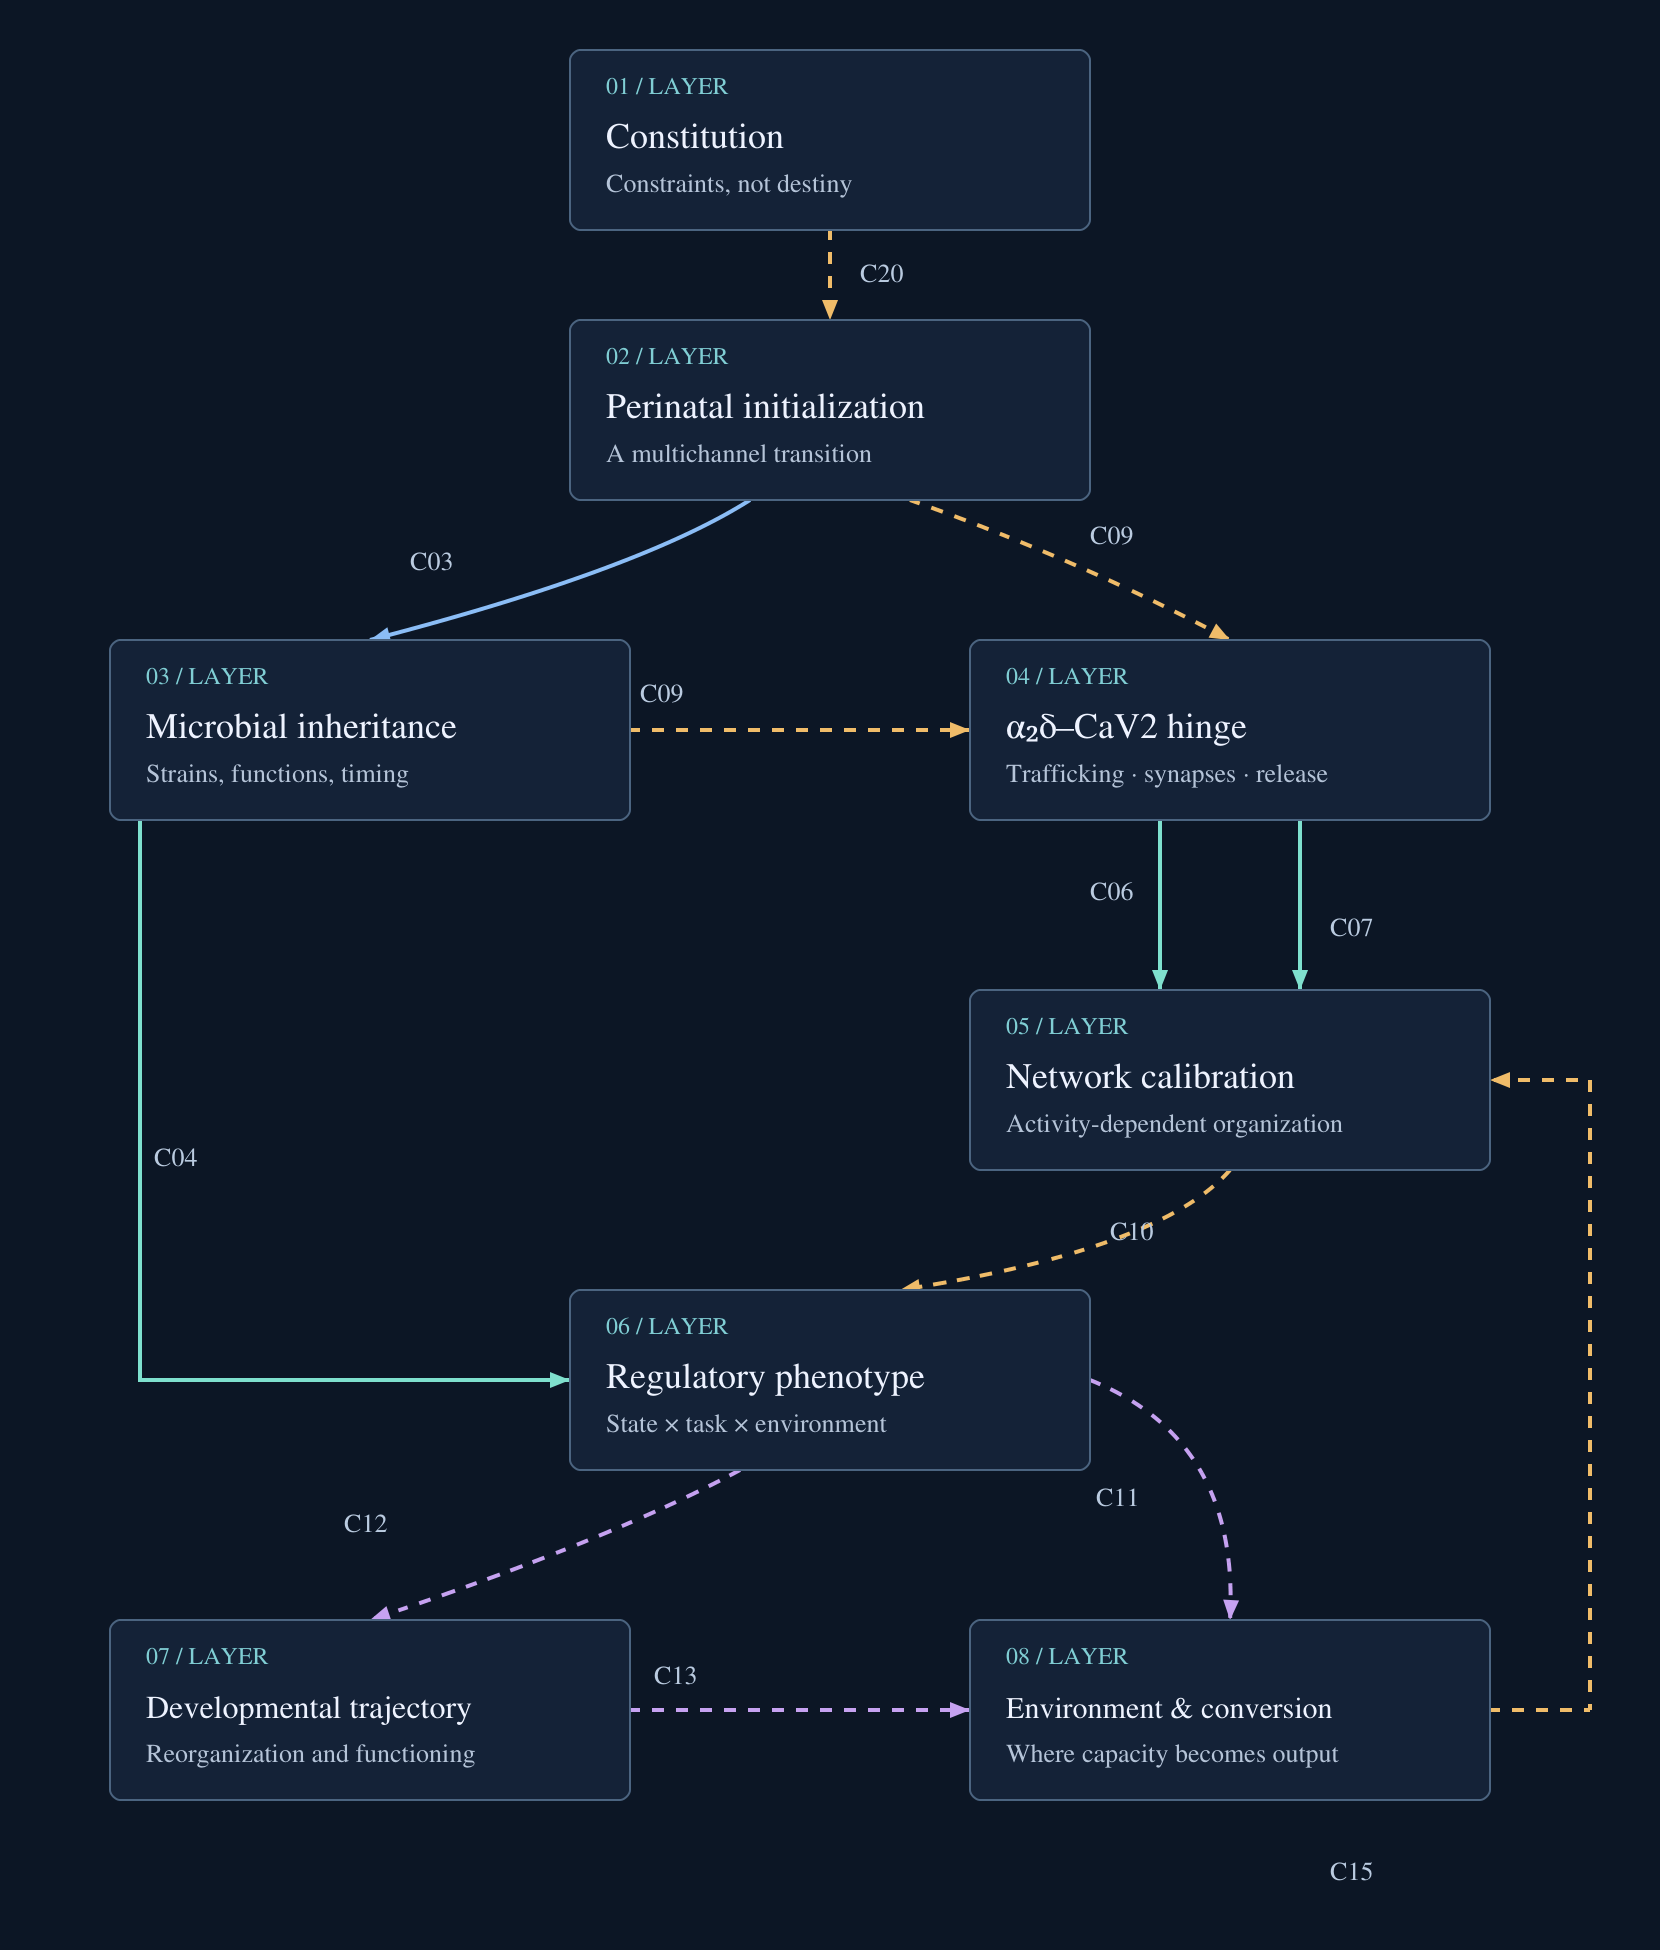
\includegraphics[height=5.6in,keepaspectratio]{../../assets/master-map.png}
\caption{Evidence-graded master field. Solid links concern bounded evidence; dashed links mark proposed bridges or horizon claims. Connection IDs resolve to the claim ledger. Feedback is indexed across time.}
\label{fig:master}
\end{figure*}

\section{Perinatal pathways}

\subsection{Perinatal Regulatory Initialization}

PRI describes the transition from intrauterine regulation to respiration, feeding, temperature control, microbial acquisition, and social contact. Birth mode is an imperfect proxy for that multidimensional transition. Labor before caesarean delivery, surgical indication, gestational age, anesthesia, antibiotics, maternal illness, and postnatal care must be distinguished.

Human birth studies support large delivery-associated differences in vasopressin/copeptin. Wellmann et al. reported median arterial cord copeptin of 1,610 pmol/L after vaginal delivery versus 8 pmol/L after primary caesarean delivery in their cohort \cite{ref1}. This numerical contrast is specific to that cohort, assay, specimen, and time point. It establishes neither persistent hormonal deficiency nor a developmental effect of a specified magnitude.

A later prospective study explicitly found a birth-stress response for vasopressin but not oxytocin \cite{ref2}. The extension's broad grouping of all birth hormones must therefore be narrowed: AVP and OXT are distinct signals, and peripheral OXT is not a direct measurement of central affiliative circuitry. PRI predicts that timing and resolution of perturbation may matter; it does not imply that more stress is beneficial or that less stress is pathological.


\subsection{Maternal microbial inheritance}

Infant microbial assembly reflects multiple reservoirs and repeated exposures. Sinha et al.'s 2026 longitudinal study examined 714 mother–infant pairs and 4,526 samples, identifying the maternal gut as a major source of infant gut strains and associations with delivery and feeding \cite{ref3}. This supports a transmission ecology rather than a vaginal-canal-only model.

The causal variable proposed here is acquisition and persistence of particular organisms or functions, measured longitudinally. “Caesarean” and “vaginal” cannot substitute for those measurements. Antibiotics, diet, gestational maturity, household contacts, illness, and feeding can influence both microbial assembly and subsequent development. Stool non-detection is also not equivalent to biological absence at all mucosal sites.

Claims that a fixed percentage of modern humans has lost \emph{L. reuteri} are omitted because comparable populations, assay sensitivity, specimen sites, and strains have not been harmonized in this synthesis. A decline narrative is unnecessary for testing whether a particular strain or metabolic function affects a defined outcome.


\subsection{\emph{L. reuteri}, vagal signaling, oxytocin, and social reward}

In several mouse models, Sgritta et al. linked \emph{L. reuteri}-associated changes in social behavior to an intact vagus, oxytocin signaling, and social-interaction-related plasticity in ventral tegmental area circuitry \cite{ref4}. This is experimentally informative preclinical evidence. It is not proof that the same sequence explains human autism or that normal human development requires one commercially available strain.

Human findings remain narrower. The SB-121 crossover study enrolled 15 autistic participants aged 15–45 years, with safety as its primary objective \cite{ref5}. Adaptive-behavior signals were exploratory; the reported eye-tracking social-preference contrast had p = 0.1, and the plasma OXT contrast had p = 0.106. Neither constitutes a conventionally significant demonstration of the proposed human mediator. Multiple exploratory outcomes and formulation-specific effects limit interpretation.

A separate pediatric pilot trial reported improved social behavior without improvement in overall autism severity \cite{ref6}. This is compatible with dimensional specificity but does not establish developmental origin, vagal mediation, or \ensuremath{\alpha_2\delta} involvement. The key distinction is between a human intervention signal and verification of the full animal-derived pathway. A negative global autism endpoint must remain visible beside any positive social endpoint.


\subsection{Behavioral immune and disgust calibration}

The extension proposes two partially separable dimensions: affiliative/social-reward sensitivity and defensive pathogen-avoidance sensitivity. A schematic response model is Social approach = \ensuremath{\alpha} \ensuremath{\times} affiliative gain − \ensuremath{\beta} \ensuremath{\times} avoidance gain + contextual terms. The coefficients are not estimated and the dimensions need not be opposites; affiliation and pathogen avoidance can both be high.

The proposed bridge from early microbial/immune conditions to later germ aversion is E0. The Howard et al. meta-analysis distinguishes perceived infectability from germ aversion and reports different relationships with disgust and outgroup perceptions \cite{ref7}. It does not test PRI. Culture, threat learning, social experience, and measurement overlap provide competing explanations.

Disgust sensitivity and germ-aversion calibration are therefore a secondary horizon track. It must first predict age-appropriate contamination-avoidance measures before any broader social interpretation is attempted. Birth mode, microbiome status, diagnosis, or receptor state cannot be used to infer an individual's ideology, morality, or attitudes toward other people.

\section{Molecular and constitutional mechanisms}

\subsection{CACNA1B and the developmental role of CaV2.2}

CACNA1B encodes the pore-forming component of CaV2.2, an N-type calcium channel implicated in presynaptic release. CaV2.1, encoded by CACNA1A, is another major release channel. Channel contributions vary across neurons, compartments, developmental stages, and preparations.

Rat auditory-brainstem experiments demonstrate developmental changes in the channel types supporting transmission \cite{ref8}. These data justify a synapse-specific handoff visualization, not a universal schedule in which an immature brain is CaV2.2 and a mature brain is CaV2.1. A different preparation may retain substantial N-type contribution; absence of the illustrated switch need not mean arrested development.

Human biallelic CACNA1B loss-of-function variants were reported in a severe epilepsy–dyskinesia syndrome \cite{ref9}. This demonstrates that major disruption can matter profoundly. It does not show that ordinary birth variation produces a smaller version of the same syndrome. The proposed environmental bridge needs direct evidence in a biologically plausible exposure range. Hypoxia-specific CACNA1B splice claims and a birth-trauma-induced universal stalled switch are not asserted.


\subsection{The \ensuremath{\alpha_2\delta} / CACNA2D developmental hinge}

The \ensuremath{\alpha_2\delta} family supplies a particularly informative interface because trafficking and synapse organization can be experimentally separated. Eroglu et al. identified \ensuremath{\alpha_2\delta}-1 as a neuronal thrombospondin receptor supporting excitatory synaptogenesis \cite{ref10}. Risher et al. investigated its postsynaptic Rac1-dependent synaptogenic role in developing mouse cortex \cite{ref11}. Ferron et al. experimentally connected proteolytic maturation of \ensuremath{\alpha_2\delta} with vesicular release probability \cite{ref12}.

These findings support multiple molecular functions, not a single scalar “\ensuremath{\alpha_2\delta} level.” CACNA2D1–4 encode distinct family members; results for \ensuremath{\alpha_2\delta}-1 cannot be transferred automatically to every isoform. Synaptogenic and channel-related functions can overlap without being identical. Astrocyte-dependent synapse formation should not be silently reduced to presynaptic calcium influx.

A mouse nerve-injury study found \ensuremath{\alpha_2\delta}-1-dependent CaV2.2 trafficking in selected dorsal-root neurons \cite{ref29}; that preparation is not a perinatal brain model. Mouse brain expression profiles vary by region and developmental stage, and one activity-blockade condition did not alter the measured channel-expression program \cite{ref30}. A biochemical assay found that gabapentin did not directly inhibit binding of soluble thrombospondin-4 to \ensuremath{\alpha_2\delta}-1 \cite{ref31}, even though earlier synaptogenesis experiments found drug-sensitive outcomes \cite{ref10}. The binding event, channel trafficking and downstream synapse formation therefore remain separate steps. Rare biallelic CACNA2D1 loss-of-function in two humans impaired CaV2 trafficking in assays and was associated with severe early encephalopathy \cite{ref35}; it cannot identify the effects of common variation or ordinary exposure.

The unproven bridge is explicit: do realistic endocrine, inflammatory, metabolic, or microbial perturbations alter particular \ensuremath{\alpha_2\delta} states during relevant sensitive periods, and do those changes mediate durable network differences? Hinge status would require temporal ordering, intervention, selective disruption or rescue, and a comparison with alternative pathways. A correlation between exposure and CACNA2D transcript abundance alone is insufficient.


\subsection{The RCCX constitutional interface}

The broad project hypothesis invokes immune, endocrine, and connective-tissue convergence at the RCCX region \cite{projP1}. Specific human evidence exists for contiguous CYP21A2–TNXB disruption and the CAH-X phenotype: Merke et al. documented connective-tissue manifestations associated with tenascin-X haploinsufficiency in a subset of congenital adrenal hyperplasia patients \cite{ref13}. This is a defined molecular-clinical relationship.

Additional clinical genetics work maps the RCCX structural arrangement and CAH-X testing boundary \cite{ref22}. Complement C4 variation has a distinct schizophrenia association and a mouse postnatal-pruning result \cite{ref23}, not a general RCCX developmental pathway. ADHD genome-wide analysis identified 27 risk loci \cite{ref24}, directly challenging a one-locus account. In a selected 102-person hEDS/HSD clinical cohort, 48\% met a POTS definition \cite{ref33}; this is not a population prevalence or evidence that RCCX caused the autonomic phenotype.

It must not be generalized into an established RCCX cause of autism, ADHD, overexcitability, autonomic illness, or polymathic capacity. Chromosomal proximity does not demonstrate coordinated expression, a common latent syndrome, or causal mediation through \ensuremath{\alpha_2\delta}. No direct RCCX \ensuremath{\rightarrow} \ensuremath{\alpha_2\delta} mechanism is established by the evidence used here.

The research design should compare the incremental value of prespecified RCCX variables against broader polygenic, obstetric, immune, endocrine, and connective-tissue measures. If the RCCX subset adds no replicated explanatory value, the RCCX-specific module should be rejected while the broader constitution \ensuremath{\times} development question remains testable. Defining susceptibility retrospectively from the very outcome to be explained would make the model circular.

\section{Regulatory phenotype and context}

\subsection{Network calibration and developmental experience}

Network calibration denotes measurable development of synaptic organization, release dynamics, sensory responses, and regulation under perturbation. It must be decomposed into outcomes such as evoked responses, recovery time, variability, and learning rather than inferred from a global impression of “high gain.”

Experimental rat work connects maternal care with epigenetic regulation of glucocorticoid-receptor-related stress processes \cite{ref14}. Human postmortem work associates childhood abuse history with hippocampal glucocorticoid receptor regulation \cite{ref15}. Species, tissue, developmental window, ascertainment, and causal design differ. These studies support developmental embedding as a domain of inquiry; they do not establish that the same epigenetic modification mediates the present PRI–CaV proposal or that acquired states are transmitted through the human germline.

Human stress-methylation evidence is mixed rather than a settled inheritance mechanism. In 113 mother–infant dyads, maternal maltreatment associations did not directly appear in newborn methylation at the assayed sites \cite{ref25}. A separate FKBP5 association replicated in Holocaust offspring, but the transmission route remained unresolved \cite{ref26}. In a population sample of 3,965 adults, previously reported childhood-maltreatment interactions at tested FKBP5 sites were not replicated \cite{ref34}. These studies differ in tissue, timing, cell mixture, genotype and ascertainment. They motivate prospective measurement, not an assertion that trauma is inherited as a specific methylation mark.

Autonomic variation, sleep, pain, sensory load, learned threat, and social reinforcement can change current attention without requiring an early molecular lesion. Adult autistic camouflaging has a validated self-report measure \cite{ref32}, but the broader cascade’s automatic or homeostatic masking remains a proposed transfer across phenotypes. These are competing and interacting pathways. A useful longitudinal analysis must allow compensation, recovery, nonlinear responses, and different trajectories leading to similar observed phenotypes.


\subsection{Regulatory Closure Bias: construct and operationalization}

Regulatory Coupling Orientation names the hypothesis that the relative contribution of external interaction and internally sustained stabilization varies by person, task, and state. Both are present in every person. RCB is the proposed quantitative index:

\begin{equation}
\mathrm{RCB}_{i,\tau,s}=\ln\!\left(\frac{G_{\mathrm{exo}}}{G_{\mathrm{endo}}}\right),
\qquad G_{\mathrm{exo}},G_{\mathrm{endo}}>0 .
\end{equation}

The logarithm is defined only for positive, commensurate gains. These terms must not be assigned from a diagnosis or questionnaire label. An event-rate meta-analysis found disproportionate slowing of ADHD groups under slow Go/No-Go event rates, larger commission-error effects under fast rates, and persisting general group differences; reaction-time variability did not show the predicted event-rate effect \cite{ref27}. That is a bounded task result, not a validated RCB index. One candidate protocol randomizes participants across externally responsive and internally paced conditions with matched difficulty, reward, sensory load, practice, and time on task. Predefine a regulatory error L, such as a weighted, standardized combination of performance variability and recovery following a task perturbation. Estimate condition-specific reductions relative to a common reference.

If an estimated gain is nonpositive or indistinguishable from zero, report the component estimates and their uncertainty; do not force a ratio by adding an arbitrary constant. A prespecified stabilized index may be evaluated as a separate measure but must disclose its dependence on the chosen constant. Repeated sessions should test reliability, construct validity, and incremental prediction beyond arousal, executive function, reward sensitivity, and symptom severity.

The website's positive-gain sliders illustrate the mathematics only. Their values are arbitrary teaching inputs, not normative scores, biological measurements, diagnoses, or estimated coefficients. The main empirical prediction concerns the interaction of independently measured RCB with environment; a favorable response cannot both define and validate the construct in the same data.


\subsection{Hunter/Farmer and Dąbrowski interpretations}

Hunter/Farmer terminology describes ecological renderings of behavior, not ancestral castes or fixed human types. An online foraging study linked attention-deficit traits with exploratory choices \cite{ref16}. In a different Hadza actigraphy study, one or more group members were scored awake or in light sleep in 99.8\% of sampled nighttime epochs across 20 days \cite{ref28}. This illustrates group-level chronotype heterogeneity, but did not measure ADHD, ancestral subtypes, or modern work performance. Such findings motivate task-dependent hypotheses; they do not prove an evolutionary origin of ADHD or universal advantage under uncertainty.

Dąbrowski's framework contributes a vocabulary for instability followed by reorganization \cite{ref17}. Psychomotor, sensory, emotional, intellectual, and imaginational overexcitabilities are retained as historical conceptual dimensions. They are not demonstrated consequences of RCCX or \ensuremath{\alpha_2\delta} biology. “Bifurcation” is used as a model of divergent trajectories, not an empirically identified mathematical phase transition.

The studyable question is whether particular combinations of sensitivity, context, support, and self-regulation predict improved functioning or sustained impairment. Reorganization can be multidirectional, reversible, and domain-specific. Suffering is neither necessary nor sufficient for insight; disability, originality, and achievement must be measured separately. Conversion and dissemination depend on resources and social opportunity as well as individual capacity.


\subsection{Pharmacological retrodiction: provenance, not diagnosis}

Adult reports of broad state changes following a compound can motivate a candidate mechanism. Zvejniece et al. provide experimental evidence for R-phenibut binding to \ensuremath{\alpha_2\delta} alongside its GABA-B pharmacology \cite{ref18}. This offers a reason to investigate both targets, not a way to infer which target produced a particular person's experience.

Retrodiction from an adult response to a developmental cause is underdetermined by multiple targets, kinetics, current state, expectation, and downstream network effects. Similarity of benefit does not identify a shared lesion; differences between related compounds do not uniquely isolate a target. No adult self-report is counted as evidence for PRI or \ensuremath{\alpha_2\delta} developmental pathology here. Pharmacological provenance is recorded separately from the causal ledger, without a treatment proposal or dosing protocol.

\section{Causal identification and human evidence}

\subsection{Competing explanations and causal DAGs}

The causal graphs in Figure 1 and the interactive site distinguish mechanism from confounding. Birth mode D, obstetric indication O, maternal/familial factors G, antibiotics X, microbiota M, endocrine response B, molecular state C, and outcome Y are different variables. A candidate perinatal graph contains O \ensuremath{\rightarrow} D and O \ensuremath{\rightarrow} Y; G \ensuremath{\rightarrow} D and G \ensuremath{\rightarrow} Y; D \ensuremath{\rightarrow} M and D \ensuremath{\rightarrow} B; X \ensuremath{\rightarrow} M; and the proposed M/B \ensuremath{\rightarrow} C \ensuremath{\rightarrow} Y paths. Antibiotic timing and indication can change whether X is a confounder, mediator, or co-exposure; it must not be mechanically adjusted in every analysis.

The confounding-only competitor preserves O/G \ensuremath{\rightarrow} D and O/G \ensuremath{\rightarrow} Y while deleting D-mediated paths. The bypass competitor preserves M/B \ensuremath{\rightarrow} Y while deleting C mediation. A postnatal-learning competitor attributes later regulation to ongoing environment, sleep, pain, and reinforcement with little stable contribution from PRI. The model must outperform these alternatives on held-out data and mechanistic interventions.

Xiao et al. reported fully adjusted odds ratios of 1.02 (95\% CI 0.81–1.29) for ASD and 1.06 (0.95–1.18) for ADHD in the Nurses' Health Study II analysis \cite{ref19}. These null associations constrain broad birth-mode claims. Moving to dimensional outcomes is legitimate only when outcomes and analysis are specified prospectively; otherwise it risks moving the goalposts. Sibling designs can reduce shared familial confounding but do not automatically remove nonshared confounding or measurement error.

The target total effect is E[Y under do(D=d\textsubscript{1})] − E[Y under do(D=d\textsubscript{0})], where the intervention must be well defined. For this program, contrasts in specified microbial or physiological exposures may be more interpretable than a heterogeneous delivery label. Mediated effects through C require additional assumptions about mediator–outcome confounding, exposure-induced confounding, consistency, positivity, and measurement. Conditioning on consequences such as neonatal intensive care can introduce selection or collider bias. A DAG states assumptions; it does not prove them.


\subsection{Human intervention evidence and its boundaries}

Zhou et al.'s 12-month follow-up enrolled 70 dyads in each of the VMT, saline-control, and nonrandomized vaginal-delivery reference groups \cite{ref20}. The VMT–control contrast favored the social-emotional questionnaire score (mean difference −9.24; 95\% CI −16.04 to −2.45), while the total ASQ-3 contrast was not significant (8.90; −2.9 to 20.70). The distinction between randomized treatment comparison and natural reference group is essential.

This pilot offers an intervention signal for a particular protocol and endpoint, with exploratory follow-up limitations. It neither identifies a responsible strain nor measures the \ensuremath{\alpha_2\delta} hinge. It also does not establish improved long-term functioning, a change in autism probability, or a universally beneficial microbiome. An intervention can affect a social measure through routes wholly independent of the proposed molecular mechanism. Any future neonatal intervention belongs in a formally approved trial with infection screening and safety monitoring, not an inference-driven self-experiment.


\begin{figure*}[t]
\centering
\begin{minipage}{.48\textwidth}\centering
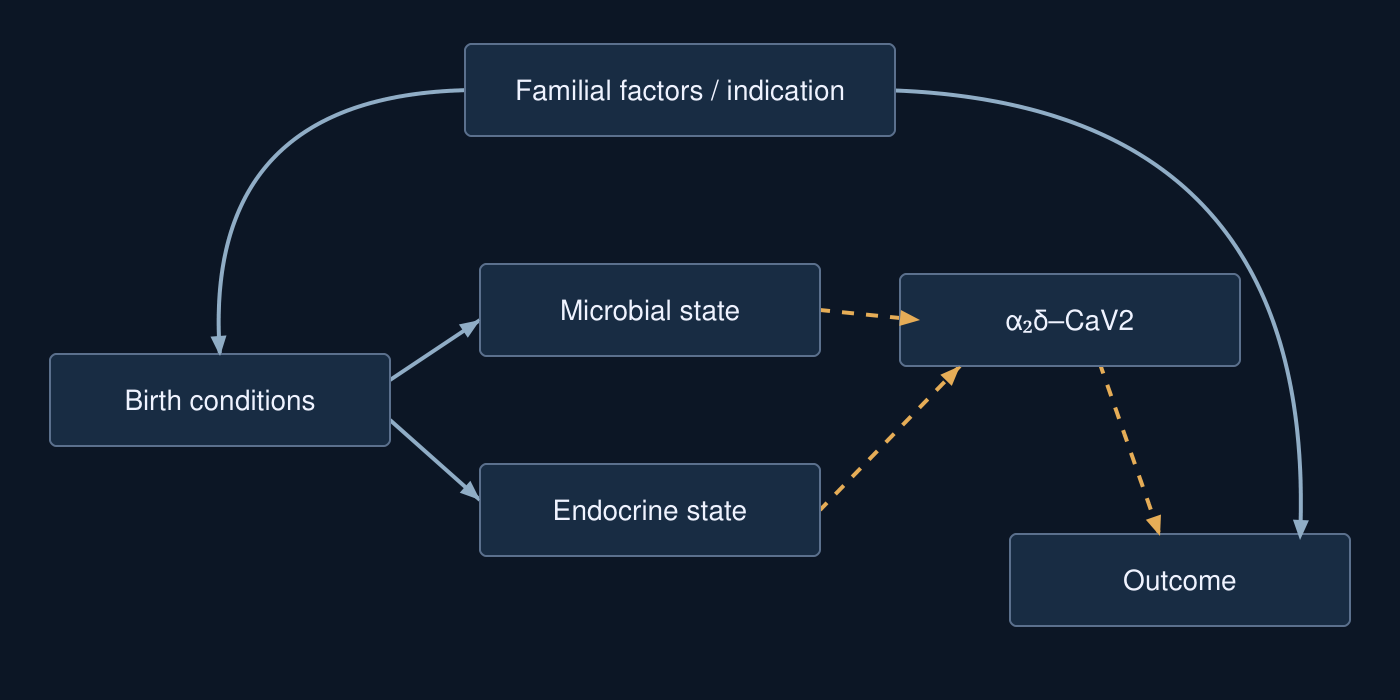
\includegraphics[width=\linewidth]{../../assets/dag-integrated.png}\\
\small (a) Candidate mediator
\end{minipage}\hfill
\begin{minipage}{.48\textwidth}\centering
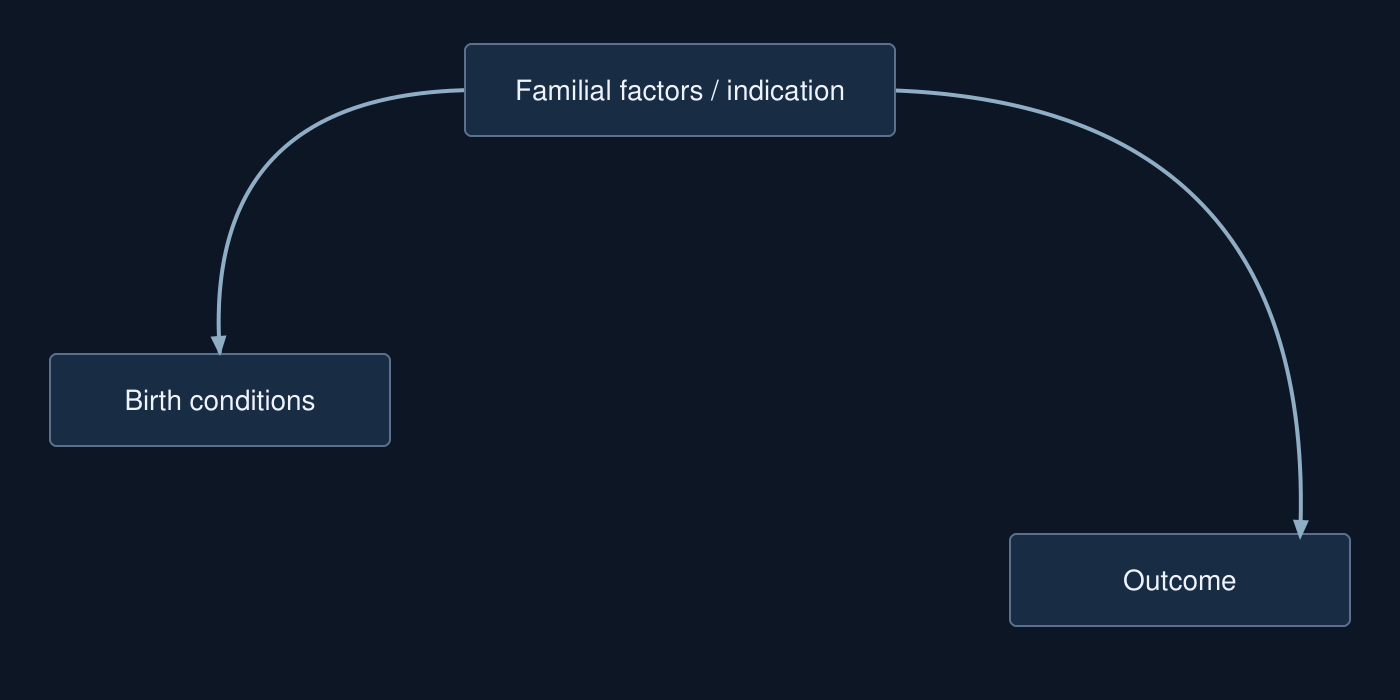
\includegraphics[width=\linewidth]{../../assets/dag-confounding.png}\\
\small (b) Confounding-only alternative
\end{minipage}\\[.8em]
\begin{minipage}{.48\textwidth}\centering
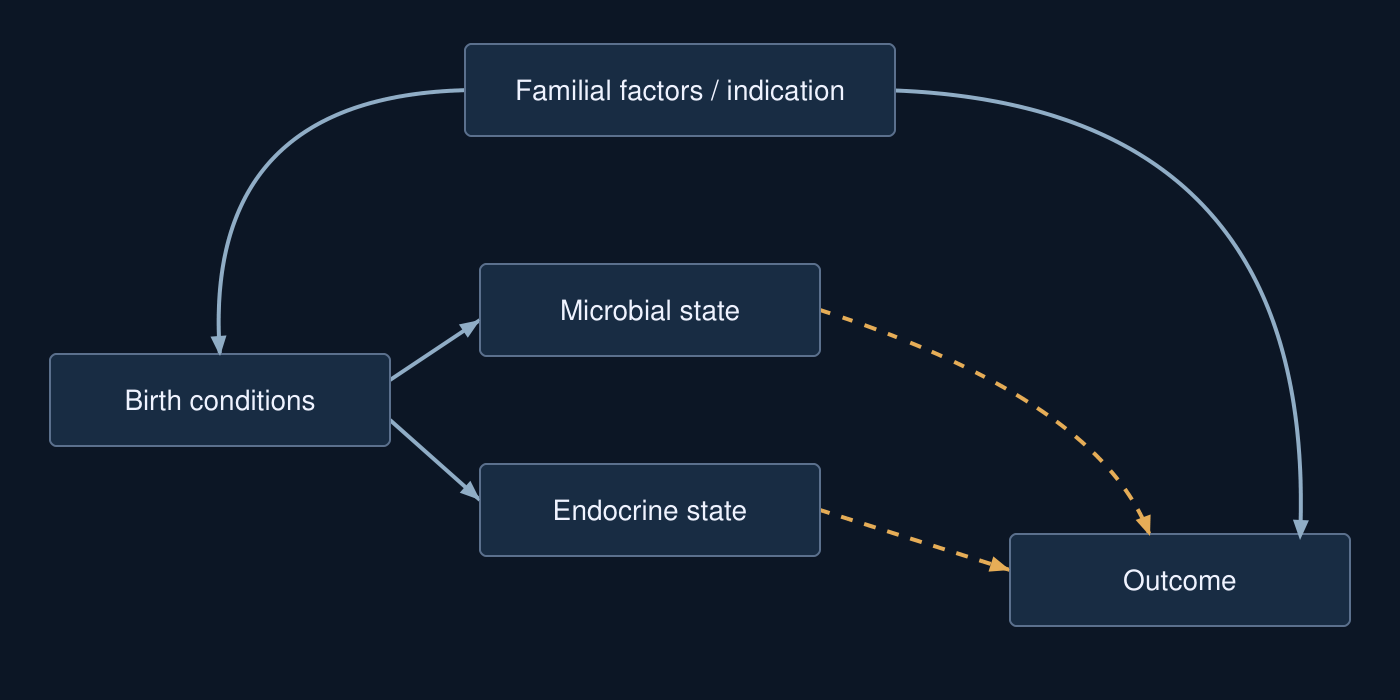
\includegraphics[width=\linewidth]{../../assets/dag-bypass.png}\\
\small (c) Hinge-bypass alternative
\end{minipage}
\caption{Competing causal architectures. The same outcome can arise with or without the candidate molecular mediator; these are study assumptions, not fitted effects.}
\label{fig:alternatives}
\end{figure*}

\section{Predictions and discriminating studies}

\subsection{Falsifiable predictions}

P1: A prespecified, physiologically justified early perturbation changes a defined \ensuremath{\alpha_2\delta}/CaV measure before a network outcome changes. A sufficiently precise null across the nominated window weakens that specific bridge. P2: Selective perturbation or rescue of that measure changes the exposure's network effect. Persistence of the full effect despite successful mediator manipulation favors a bypass explanation.

P3: Measured strain acquisition or function improves prospective prediction of selected developmental dimensions beyond delivery label, covariates, and sampling artifacts. Failure on a held-out cohort rejects the nominated microbial contribution; it does not license switching organisms after seeing the outcome. P4: Constitutional effect modification replicates for predefined markers. A null interaction with adequate precision weakens the named susceptibility model.

P5: Independently estimated RCB predicts differential response to responsive versus internally paced work environments. Failure to replicate, poor reliability, or no incremental value beyond conventional measures weakens the construct. P6: AI with explicit completion constraints improves verified output differently from unconstrained AI, conditional on baseline regulatory measurements. More generated text or more branches alone does not count as improved conversion.

P7: Early microbial/immune variables predict age-appropriate germ aversion after prespecified adjustments. Failure weakens the behavioral-immune extension independently of social-reward pathways. P8: The civilization-level inversion should vary by task, opportunity, and resources. A persistent specialist advantage on depth-intensive tasks is compatible with the hypothesis; an absence of the predicted integrative-profile advantage in its nominated environments is adverse evidence.


\subsection{Minimum discriminating experimental program}

Study A: Mechanistic exposure \ensuremath{\times} mediator experiment. In a specified developing neural preparation, choose one exposure and one \ensuremath{\alpha_2\delta} mechanism before testing. Use a factorial design with exposure/control and selective mediator perturbation/control, supplemented by an orthogonal rescue. Measure viability, differentiation, channel localization, cleavage where relevant, release, and network activity in temporal order. Independent cultures or litters, rather than individual cells alone, define biological replication. Mask analysis, preregister a primary endpoint and smallest effect of interest, and justify sample size from pilot variance. This is the first gate for H1. Organoids cannot model the complete vagal–microbial loop.

Study B: Prospective mother–infant cohort. Recruit before delivery; record indication, labor, antibiotics and timing, maternal strain reservoirs, endocrine measurements with assay validation, feeding, and repeated infant strain/function measures. Predefine a small set of dimensional outcomes and a held-out validation sample. Test confounding-only, parallel-path, and candidate mediation models; use sensitivity analyses for missingness and unmeasured confounding. Accessible peripheral measures are not validated substitutes for brain \ensuremath{\alpha_2\delta} state. A cohort alone cannot close that molecular gap.

Study C: Randomized adult environment crossover. Estimate RCB in independent baseline sessions, then cross task environment with AI assistance and completion constraints. Compare blinded ratings of completed, verifiable artifacts, error burden, retention, task switching, recovery and between-team diversity. A gain in individual quality with convergence across outputs is a distinct result, not a single success score. Counterbalance order and account for learning and carryover. This study directly tests the environmental bridge and remains useful even if PRI fails.

A contingent Study D would replicate a narrowly selected microbial intervention with preregistered mediators and longer follow-up. Randomized assignment estimates the intervention effect; engraftment is post-randomization, so comparing engrafters with non-engrafters does not automatically estimate its causal effect. An animal endocrine \ensuremath{\times} microbial design can test interactions after Study A identifies a plausible molecular target, with litter, maternal-care, and surgical-procedure controls. These are proposed designs, not completed or ethically approved protocols.


\subsection{Evidence ledger}

The accompanying ledger assigns each major connection an ID, claim class, design code, preparation/developmental scope, source, unresolved inference, and falsifier. Figure 1 uses those same IDs. C01 identifies specific constitutional biology; C02 summarizes birth signaling; C03 covers microbial inheritance; C04 and C05 separate mouse social-reward mechanisms from human intervention signals; C06 and C07 distinguish synaptogenesis from release regulation; C08 bounds developmental channel reallocation; C09 marks the unproven perinatal-to-hinge bridge; C10 marks the integrated network-to-regulation inference; C11–C15 address regulatory coupling, developmental reorganization, environmental conversion, disgust, and time-indexed feedback; C16 records null epidemiology; C17 records the VMT trial; C18 isolates the unproven RCCX-to-hinge bridge; C19 preserves pharmacological provenance. C21–C27 add the later-life and counterevidence layer: mixed stress-epigenetic observations, task event-rate effects, bounded camouflaging, group chronotype heterogeneity, selected-cohort autonomic findings, the AI quality–diversity tradeoff, and rare severe CACNA2D1 functional evidence.

For proposed and horizon connections, references provide background plausibility or theory provenance, not evidence for the entire arrow. Removal of all E0 connections should visibly disconnect the complete central cascade. That disconnection is an intended demonstration of the present evidence boundary, not an interface defect.

\section{Discussion and limitations}

\subsection{Discussion: coupling to The Polymathic Singularity}

The environmental extension predicts changes in payoff, not a replacement of specialists by a superior biological type. Its useful empirical unit is a task-specific interaction: performance = person factors + environment factors + person \ensuremath{\times} environment + resource and history terms. A civilization-level claim requires repeated evidence across settings rather than extrapolation from one successful human–AI collaboration.

Doshi and Hauser's experiment found that generative-AI ideas could improve evaluated individual story creativity while reducing collective diversity \cite{ref21}. This supplies a concrete example of gains and losses occurring at different scales. It does not demonstrate a special advantage for an exoregulatory phenotype, historical selection reversal, or a completed phase transition.

The \ensuremath{\kappa} conversion ratio in the earlier papers depends on an unobserved denominator, “latent integrative capacity.” A stronger operational approach measures verified output, quality, cost, time, and completion separately; any latent-capacity estimate requires an explicit measurement model. New tools can support regulation, increase distraction, or both. The practical empirical question is which coupling conditions improve sustained functioning and durable work, for whom, and at what cost.


\subsection{Limitations}

The full chain has not been demonstrated. This narrative synthesis does not establish completeness of the literature, pooled effects, publication-bias correction, or causal identification. Some pivotal studies are small or preparation-specific, and source anchors are not interchangeable with replications. Human intervention evidence does not establish the proposed mediator. Brain molecular state is difficult to measure longitudinally in living infants, creating a substantial translational gap.

RCB, PRI as an integrated operator, the broad RCCX constitutional cluster, and the Dąbrowski-to-biology mapping remain unvalidated constructs or syntheses. Their flexibility creates a risk of post hoc accommodation; preregistered exclusions, alternative models, stopping rules, and independent replication are necessary. The framework does not explain every developmental phenotype and does not infer individual etiology from group averages. It does not support reducing clinical needs to environmental mismatch or romanticizing physiological impairment.

Historical claims about industrial institutions and future labor demand are narrower here than in the conceptual source. They remain motivating interpretations until operationalized. Bibliographic verification establishes the identity and relevance of a cited study, not a forensic audit of its raw data. Journal-specific formatting, external domain review, and an author-approved disclosure statement remain submission steps.

\section{Conclusion}

The contribution is a causal research architecture with separable commitments. Constitution provides candidate constraints; PRI identifies an early measurement interval; \ensuremath{\alpha_2\delta}–CaV2 biology supplies experimentally tractable mechanisms; network and regulatory measures connect development to present function; environmental coupling tests how that function changes across conditions. The decisive missing evidence lies in the bridges, especially physiologically realistic perinatal perturbation \ensuremath{\rightarrow} molecular state \ensuremath{\rightarrow} durable network effect.

Making these gaps explicit strengthens the program. It permits direct tests, isolates failures, and prevents established molecular biology from lending unearned certainty to a broad developmental narrative. The central question is which coupled developmental processes change the probability of later regulatory trajectories, and which environments allow those trajectories to produce stable, meaningful action.

\section*{Declarations and provenance}

This article reports no new human or animal experiment. The conceptual framework is attributed to E. T. Ellis; manuscript synthesis, literature assistance, and the interactive implementation were prepared with OpenAI Codex. The author should review the final wording and disclosures before journal submission. Funding and competing-interest declarations are not inferred from missing information. The two original PDFs and extension are retained as dated source artifacts. The new paper, diagrams, and machine-readable evidence ledger are versioned together. Illustrative controls contain no fitted biological parameters.

\appendix
\section{Claim-level evidence ledger}
Status and design code are separate. An E0 citation supplies background or provenance without establishing the whole bridge.
\subsection*{C01 · Specific constitutional variants \ensuremath{\rightarrow} tissue phenotype}
\noindent\textbf{Supported · E1 · Human CAH-X genotype–phenotype cohort}\par
\textit{Claim.} CYP21A2–TNXB disruption supplies a defined endocrine/connective-tissue interface.\par
\textit{Limit.} This does not validate the broad RCCX neurodevelopmental cluster. The autonomic frequency in selected hEDS/HSD clinics cannot be generalized to all carriers.\par
\textit{Rival.} Other genetic and clinical pathways explain similar tissue findings outside CAH-X.\par
\textit{Discriminator.} A prespecified RCCX contribution must add replicated prediction beyond broader constitutional measures.\par
\textit{Sources.} \cite{ref13,projP1,ref22,ref33}\par
\subsection*{C02 · Birth conditions \ensuremath{\rightarrow} AVP / copeptin response}
\noindent\textbf{Supported · E2 · Human newborn cord blood}\par
\textit{Claim.} Delivery-associated AVP/copeptin differences are reported across human studies.\par
\textit{Limit.} An acute peripheral signal does not establish persistent neural calibration; OXT is not interchangeable.\par
\textit{Rival.} Obstetric indication and the acute transition explain the cord signal without lasting calibration.\par
\textit{Discriminator.} A persistent-developmental claim needs longitudinal effects beyond the transient birth response.\par
\textit{Sources.} \cite{ref1,ref2}\par
\subsection*{C03 · Maternal ecology \ensuremath{\rightarrow} infant strain inheritance}
\noindent\textbf{Supported · E1 · Human mother–infant longitudinal cohort}\par
\textit{Claim.} Maternal gut reservoirs, delivery, feeding and subsequent contacts shape measured strain acquisition.\par
\textit{Limit.} Delivery label is a proxy; observational transmission does not establish a behavioral effect.\par
\textit{Rival.} Delivery mode is a marker for feeding, maternal reservoirs, antibiotics, and household ecology.\par
\textit{Discriminator.} The nominated strain/function fails to add held-out prediction of prespecified outcomes.\par
\textit{Sources.} \cite{ref3}\par
\subsection*{C04 · \emph{L. reuteri} \ensuremath{\rightarrow} vagus / OXT / VTA social plasticity}
\noindent\textbf{Established · E3 · Mouse ASD-related models}\par
\textit{Claim.} Vagal integrity and oxytocin signaling participate in experimentally observed social-behavior rescue.\par
\textit{Limit.} The complete pathway has not been causally demonstrated in humans.\par
\textit{Rival.} Other microbial metabolites or immune routes mediate the mouse social effect.\par
\textit{Discriminator.} Replicated pathway-specific disruption fails to alter the effect in the nominated preparation.\par
\textit{Sources.} \cite{ref4}\par
\subsection*{C05 · \emph{L. reuteri} formulation \ensuremath{\rightarrow} selected human outcomes}
\noindent\textbf{Supported · E4 · Pilot trials: children; adolescents/adults}\par
\textit{Claim.} Human trials provide limited social or adaptive-behavior signals.\par
\textit{Limit.} Global autism severity is not consistently improved; human OXT/vagus mediation remains unproven.\par
\textit{Rival.} Trial-specific formulation effects, chance, or multiple endpoints explain the selected benefit.\par
\textit{Discriminator.} Adequately powered replication fails on prespecified social outcomes.\par
\textit{Sources.} \cite{ref5,ref6}\par
\subsection*{C06 · Thrombospondin–\ensuremath{\alpha_2\delta}-1 \ensuremath{\rightarrow} synaptogenesis}
\noindent\textbf{Established · E3 · Rodent neural preparations and developing mouse cortex}\par
\textit{Claim.} \ensuremath{\alpha_2\delta}-1 participates in excitatory synapse formation; postsynaptic Rac1 is mechanistically implicated.\par
\textit{Limit.} Not identical to presynaptic trafficking; not a demonstrated consequence of birth mode. A later binding assay found soluble TSP4–\ensuremath{\alpha_2\delta}-1 binding was gabapentin-insensitive; binding and synapse outcomes must be separated.\par
\textit{Rival.} Thrombospondin signaling acts through downstream partners independently of CaV trafficking.\par
\textit{Discriminator.} Orthogonal replication fails for the specified receptor-dependent synaptogenic effect.\par
\textit{Sources.} \cite{ref10,ref11,ref31}\par
\subsection*{C07 · \ensuremath{\alpha_2\delta} maturation \ensuremath{\rightarrow} release regulation}
\noindent\textbf{Established · E3 · Experimentally manipulated neuronal culture}\par
\textit{Claim.} Proteolytic maturation of \ensuremath{\alpha_2\delta} affects channel association and vesicular release probability.\par
\textit{Limit.} No verified human perinatal cleavage abnormality is inferred.\par
\textit{Rival.} Other maturation proteins or activity-dependent changes explain release regulation.\par
\textit{Discriminator.} Selective maturation manipulation fails to reproduce the release effect in the claimed preparation.\par
\textit{Sources.} \cite{ref12}\par
\subsection*{C08 · Development \ensuremath{\rightarrow} channel contribution reallocation}
\noindent\textbf{Established · E3 · Rat auditory brainstem, postnatal days 4–14}\par
\textit{Claim.} Presynaptic channel contributions change during development in the studied synapse.\par
\textit{Limit.} Not a universal brain switch, a human-age calibration, or proof of arrested development. Mouse expression profiling found stage- and region-specific programs; one activity-blockade condition did not alter the measured expression profile.\par
\textit{Rival.} Intrinsic developmental programs explain the channel shift without the nominated exposure.\par
\textit{Discriminator.} Within-preparation replication contradicts the specified temporal change.\par
\textit{Sources.} \cite{ref8,ref30}\par
\subsection*{C09 · Perinatal signals \ensuremath{\rightarrow} \ensuremath{\alpha_2\delta}–CaV2 state}
\noindent\textbf{Proposed · E0 · Target developmental stage must be specified}\par
\textit{Claim.} Endocrine, immune or microbial signals might alter channel organization and synaptogenesis.\par
\textit{Limit.} This is the main missing bridge. Molecular plausibility does not demonstrate it.\par
\textit{Rival.} Early exposure affects networks through a pathway that bypasses \ensuremath{\alpha_2\delta}/CaV2.\par
\textit{Discriminator.} Precise null exposure effects, or failed mediator disruption/rescue, weaken the nominated bridge.\par
\textit{Sources.} \cite{projP3,ref10,ref12}\par
\subsection*{C10 · Network calibration \ensuremath{\rightarrow} regulatory phenotype}
\noindent\textbf{Proposed · E0 · Cross-level developmental hypothesis}\par
\textit{Claim.} Synaptic organization may influence later sensory, autonomic and affiliative regulation.\par
\textit{Limit.} The integrated mapping lacks direct longitudinal validation; many bypasses are possible.\par
\textit{Rival.} Ongoing sleep, pain, reward and social learning explain later regulation without an early molecular mediator.\par
\textit{Discriminator.} The specified network measures fail to predict or mediate the targeted outcome.\par
\textit{Sources.} \cite{projP1,projP3,ref9,ref14,ref15}\par
\subsection*{C11 · Regulatory phenotype \ensuremath{\times} environment \ensuremath{\rightarrow} closure}
\noindent\textbf{Horizon · E0 · Proposed repeated human task measures}\par
\textit{Claim.} RCB compares positive external and internal regulatory gains on the same scale.\par
\textit{Limit.} Not a validated trait, diagnosis, or normative scoring tool.\par
\textit{Rival.} Conventional arousal, executive function or reward sensitivity explains task-dependent gains.\par
\textit{Discriminator.} Poor reliability or no incremental out-of-sample interaction beyond conventional measures.\par
\textit{Sources.} \cite{projP1,projP2,ref16}\par
\subsection*{C12 · Regulation + context \ensuremath{\rightarrow} developmental reorganization}
\noindent\textbf{Horizon · E0 · Dąbrowski-inspired developmental interpretation}\par
\textit{Claim.} Different support and load trajectories may produce recovery, reorganization or persistent impairment.\par
\textit{Limit.} The bifurcation is not an established biological stage model; outcomes are not moral ranks.\par
\textit{Rival.} Resources, support and treatment explain trajectories without a discrete reorganization process.\par
\textit{Discriminator.} Operationalized trajectories fail to replicate or the construct adds no value over alternatives.\par
\textit{Sources.} \cite{projP1,ref17}\par
\subsection*{C13 · Human–AI coupling \ensuremath{\rightarrow} conversion and dissemination}
\noindent\textbf{Horizon · E0 · Proposed task- and resource-dependent interaction}\par
\textit{Claim.} Responsive tools may reduce implementation costs but can increase branching and dependence.\par
\textit{Limit.} AI writing evidence does not establish an RCB-specific advantage or civilizational inversion.\par
\textit{Rival.} Generic AI assistance and unequal opportunity explain output changes without phenotype-specific selection.\par
\textit{Discriminator.} Independent RCB fails to predict the nominated environment interaction on verified completed output.\par
\textit{Sources.} \cite{projP2,ref21}\par
\subsection*{C14 · Early immune ecology \ensuremath{\rightarrow} disgust sensitivity calibration}
\noindent\textbf{Horizon · E0 · Unverified developmental bridge}\par
\textit{Claim.} Early immune/microbial conditions might influence later pathogen avoidance.\par
\textit{Limit.} Adult disgust associations do not establish early microbial causation or political consequences.\par
\textit{Rival.} Current learning and culture explain disgust variation without early microbial calibration.\par
\textit{Discriminator.} No replicated prospective relationship with age-appropriate germ-aversion measures.\par
\textit{Sources.} \cite{projP3,ref7}\par
\subsection*{C15 · Phenotype \ensuremath{\rightarrow} selected environment \ensuremath{\rightarrow} later phenotype}
\noindent\textbf{Proposed · E0 · Time-indexed feedback hypothesis}\par
\textit{Claim.} Actions change subsequent exposure, reinforcement and support, feeding into later regulation.\par
\textit{Limit.} A cyclic diagram is not an identified causal model; time-order and confounding matter.\par
\textit{Rival.} Stable traits and environments jointly cause behavior and exposure without strong selection feedback.\par
\textit{Discriminator.} Time-indexed interventions and predictions fail against a nonfeedback alternative.\par
\textit{Sources.} \cite{projP1,projP2}\par
\subsection*{C16 · Birth mode \ensuremath{\rightarrow} categorical ASD / ADHD}
\noindent\textbf{Supported · E1 · Human observational counterevidence}\par
\textit{Claim.} Fully adjusted NHS II estimates are compatible with no association.\par
\textit{Limit.} Null categorical effects constrain broad claims; they do not test every dimensional mediator.\par
\textit{Rival.} Confounding explains crude birth-mode associations; adjusted categorical effects are near null.\par
\textit{Discriminator.} A well-identified replicated causal estimate would change this assessment.\par
\textit{Sources.} \cite{ref19}\par
\subsection*{C17 · VMT assignment \ensuremath{\rightarrow} 12-month social-emotional score}
\noindent\textbf{Supported · E4 · Pilot infant trial}\par
\textit{Claim.} Randomized VMT versus saline favored a social-emotional score; global ASQ-3 was not significant.\par
\textit{Limit.} No identified strain or \ensuremath{\alpha_2\delta} mediator; vaginal reference group was not randomized.\par
\textit{Rival.} The intervention affects social scores through a pathway independent of the named organism or molecular hinge.\par
\textit{Discriminator.} Larger preregistered replication fails to confirm the specific outcome.\par
\textit{Sources.} \cite{ref20}\par
\subsection*{C18 · RCCX susceptibility \ensuremath{\rightarrow} \ensuremath{\alpha_2\delta} hinge}
\noindent\textbf{Proposed · E0 · No direct evidence located in this pass}\par
\textit{Claim.} Constitution could modify sensitivity to developmental perturbation.\par
\textit{Limit.} Specific RCCX-to-channel mediation is unproven; genomic proximity is insufficient. ADHD GWAS is polygenic; a C4 schizophrenia result does not establish this neurodevelopmental bridge.\par
\textit{Rival.} Distributed genetic architecture and independent perinatal factors explain the data without an RCCX–hinge link.\par
\textit{Discriminator.} No prespecified RCCX interaction or incremental prediction in independent cohorts.\par
\textit{Sources.} \cite{projP1,projP3,ref13,ref22,ref23,ref24}\par
\subsection*{C19 · Phenibut pharmacology \ensuremath{\rightarrow} hypothesis generation}
\noindent\textbf{Established · E3 · Experimental binding and animal pharmacology}\par
\textit{Claim.} R-phenibut has \ensuremath{\alpha_2\delta} and GABA-B pharmacological activity.\par
\textit{Limit.} Adult response does not diagnose a target-specific or developmental lesion.\par
\textit{Rival.} GABA-B effects, expectancy, or current state explain an adult response without developmental \ensuremath{\alpha_2\delta} pathology.\par
\textit{Discriminator.} The developmental inference is not identified by a response; it requires independent tests.\par
\textit{Sources.} \cite{ref18,projP3}\par
\subsection*{C20 · Constitution \ensuremath{\times} perinatal conditions \ensuremath{\rightarrow} initialization}
\noindent\textbf{Proposed · E0 · Unverified integrated developmental interaction}\par
\textit{Claim.} Measured constitutional factors may change responses to perinatal exposures.\par
\textit{Limit.} The broad interaction is not established by CAH-X or molecular synapse studies.\par
\textit{Rival.} Constitution and perinatal conditions contribute additively, with no specific interaction.\par
\textit{Discriminator.} Prespecified constitutional effect modification fails in adequately precise independent studies.\par
\textit{Sources.} \cite{projP1,projP3,ref13}\par
\subsection*{C21 · Early adversity \ensuremath{\leftrightarrow} stress-regulatory methylation}
\noindent\textbf{Supported · E1 · Human postmortem and blood observational studies; tissue and age differ}\par
\textit{Claim.} Adversity history is associated with some NR3C1 or FKBP5 methylation and expression measures in selected samples.\par
\textit{Limit.} A 113-dyad study found no direct transfer at assayed newborn sites, and a 3,965-person population study did not replicate a maltreatment interaction. This cannot identify a universal inherited mark.\par
\textit{Rival.} Genotype, cell mixture, current illness, shared environment, and selection explain the associations.\par
\textit{Discriminator.} Prospective, cell-composition-aware replication should show the nominated site and direction across independent cohorts.\par
\textit{Sources.} \cite{ref15,ref25,ref26,ref34}\par
\subsection*{C22 · Task event rate \ensuremath{\rightarrow} attention performance}
\noindent\textbf{Supported · E2 · Go/No-Go ADHD task meta-analysis; not a general personality scale}\par
\textit{Claim.} Slow event rates disproportionately slowed ADHD groups; fast rates increased commission-error effects in the reviewed tasks.\par
\textit{Limit.} General ADHD–control differences persisted and reaction-time variability did not show the predicted event-rate effect.\par
\textit{Rival.} Specific task learning or reward expectations, rather than regulatory closure, explain the pattern.\par
\textit{Discriminator.} Matched within-person task crossovers fail to reproduce event-rate interactions beyond task demands.\par
\textit{Sources.} \cite{ref27}\par
\subsection*{C23 · Camouflaging is measurable; broad masking remains a bridge}
\noindent\textbf{Supported · E1 · Autistic adult psychometric samples}\par
\textit{Claim.} The CAT-Q measured reported social camouflaging in autistic and non-autistic adults.\par
\textit{Limit.} This does not prove unconscious homeostatic masking across ADHD, trauma, or other phenotypes.\par
\textit{Rival.} Conventional social adaptation and context account for reported strategies.\par
\textit{Discriminator.} Longitudinal behavioral and physiological measures fail to distinguish generalized masking from social learning.\par
\textit{Sources.} \cite{ref32}\par
\subsection*{C24 · Chronotype diversity \ensuremath{\rightarrow} group-level nighttime coverage}
\noindent\textbf{Supported · E1 · Hadza actigraphy, 20 days; no ADHD measure}\par
\textit{Claim.} At least one group member was scored awake or in light sleep in 99.8\% of sampled nighttime epochs.\par
\textit{Limit.} The result supports group-level heterogeneity, not an ADHD subtype or general adaptive superiority.\par
\textit{Rival.} Age structure and ordinary awakenings explain the coverage without a specialized vigilance trait.\par
\textit{Discriminator.} Comparable groups with mixed age and chronotype fail to show the predicted coverage.\par
\textit{Sources.} \cite{ref28}\par
\subsection*{C25 · Hypermobility cohorts show heterogeneous autonomic profiles}
\noindent\textbf{Supported · E1 · Selected 102-person hEDS/HSD adult clinical cohort}\par
\textit{Claim.} Autonomic testing identified varied profiles including POTS in 48\% of this selected sample.\par
\textit{Limit.} The figure is not a general-population prevalence and does not demonstrate RCCX, perinatal or \ensuremath{\alpha_2\delta} mediation.\par
\textit{Rival.} Referral selection and comorbidity explain the high clinical frequency.\par
\textit{Discriminator.} Population-based cohorts fail to reproduce an autonomic association under prespecified diagnostic criteria.\par
\textit{Sources.} \cite{ref33}\par
\subsection*{C26 · AI ideas \ensuremath{\rightarrow} individual story gains and collective similarity}
\noindent\textbf{Established · E4 · Randomized short-story writing experiment}\par
\textit{Claim.} Access to AI ideas improved average rated stories while AI-assisted stories were more similar to each other.\par
\textit{Limit.} The study does not establish benefit for scientific discovery, integrative phenotypes, or society-wide change.\par
\textit{Rival.} Task-specific anchoring explains similarity without a general AI effect.\par
\textit{Discriminator.} Preregistered replication on completed research artifacts finds no individual-quality or diversity contrast.\par
\textit{Sources.} \cite{ref21}\par
\subsection*{C27 · Severe CACNA2D1 loss \ensuremath{\rightarrow} impaired CaV2 function}
\noindent\textbf{Supported · E3 · Two rare human cases plus functional assays}\par
\textit{Claim.} Biallelic loss-of-function variants were linked to early epileptic encephalopathy and impaired CaV2 trafficking in assays.\par
\textit{Limit.} Rare severe variants do not identify effects of common variation or ordinary perinatal exposure.\par
\textit{Rival.} Other variants or pathways explain the clinical phenotype in these cases.\par
\textit{Discriminator.} Independent variant studies and orthogonal functional assays fail to reproduce the trafficking deficit.\par
\textit{Sources.} \cite{ref35}\par

\begin{thebibliography}{99}

\small

\bibitem{ref1} Wellmann S, et al. (2010). High copeptin concentrations in umbilical cord blood after vaginal delivery and birth acidosis. Journal of Clinical Endocrinology \& Metabolism. 95(11):5091–5096. \href{https://doi.org/10.1210/jc.2010-1331}{doi:jc.2010-1331}

\bibitem{ref2} Fill Malfertheiner S, et al. (2021). Vasopressin but Not Oxytocin Responds to Birth Stress in Infants. Frontiers in Neuroscience. 15:718056. \href{https://doi.org/10.3389/fnins.2021.718056}{doi:fnins.2021.718056}

\bibitem{ref3} Sinha T, et al. (2026). Maternal influences on infant gut microbiome and health. Nature. Published online 12 August 2026. \href{https://doi.org/10.1038/s41586-026-10922-9}{doi:s41586-026-10922-9}

\bibitem{ref4} Sgritta M, et al. (2019). Mechanisms Underlying Microbial-Mediated Changes in Social Behavior in Mouse Models of Autism Spectrum Disorder. Neuron. 101(2):246–259.e6. \href{https://pubmed.ncbi.nlm.nih.gov/30522820/}{PMID:30522820}

\bibitem{ref5} Schmitt LM, et al. (2023). Results of a phase Ib study of SB-121, an investigational probiotic formulation, a randomized controlled trial in participants with autism spectrum disorder. Scientific Reports. 13:5192. \href{https://doi.org/10.1038/s41598-023-30909-0}{doi:s41598-023-30909-0}

\bibitem{ref6} Mazzone L, et al. (2024). Precision microbial intervention improves social behavior but not autism severity: A pilot double-blind randomized placebo-controlled trial. Cell Host \& Microbe. 32(1):106–116.e6. \href{https://pubmed.ncbi.nlm.nih.gov/38113884/}{PMID:38113884}

\bibitem{ref7} Howard MC, Davis MM, Serviss E. (2026). A meta-analysis of perceived infectability, germ aversion, disgust and outgroup perceptions: Evaluating research on the behavioural immune system. British Journal of Psychology. Published online 18 April 2026. \href{https://doi.org/10.1111/bjop.70076}{doi:bjop.70076}

\bibitem{ref8} Iwasaki S, Takahashi T. (1998). Developmental changes in calcium channel types mediating synaptic transmission in rat auditory brainstem. Journal of Physiology. 509(Pt 2):419–423. \href{https://pubmed.ncbi.nlm.nih.gov/9575291/}{PMID:9575291}

\bibitem{ref9} Gorman KM, et al. (2019). Bi-allelic Loss-of-Function CACNA1B Mutations in Progressive Epilepsy-Dyskinesia. American Journal of Human Genetics. 104:948–956. \href{https://pubmed.ncbi.nlm.nih.gov/30982612/}{PMID:30982612}

\bibitem{ref10} Eroglu C, et al. (2009). Gabapentin receptor \ensuremath{\alpha_2\delta}-1 is a neuronal thrombospondin receptor responsible for excitatory CNS synaptogenesis. Cell. 139(2):380–392. \href{https://doi.org/10.1016/j.cell.2009.09.025}{doi:j.cell.2009.09.025}

\bibitem{ref11} Risher WC, et al. (2018). Thrombospondin receptor \ensuremath{\alpha_2\delta}-1 promotes synaptogenesis and spinogenesis via postsynaptic Rac1. Journal of Cell Biology. 217(10):3747–3765. \href{https://pubmed.ncbi.nlm.nih.gov/30054448/}{PMID:30054448}

\bibitem{ref12} Ferron L, Kadurin I, Dolphin AC. (2018). Proteolytic maturation of \ensuremath{\alpha_2\delta} controls the probability of synaptic vesicular release. eLife. 7:e37507. \href{https://doi.org/10.7554/eLife.37507}{doi:eLife.37507}

\bibitem{ref13} Merke DP, et al. (2013). Tenascin-X haploinsufficiency associated with Ehlers-Danlos syndrome in patients with congenital adrenal hyperplasia. Journal of Clinical Endocrinology \& Metabolism. 98(2):E379–E387. \href{https://pubmed.ncbi.nlm.nih.gov/23284009/}{PMID:23284009}

\bibitem{ref14} Weaver ICG, et al. (2004). Epigenetic programming by maternal behavior. Nature Neuroscience. 7:847–854. \href{https://doi.org/10.1038/nn1276}{doi:nn1276}

\bibitem{ref15} McGowan PO, et al. (2009). Epigenetic regulation of the glucocorticoid receptor in human brain associates with childhood abuse. Nature Neuroscience. 12:342–348. \href{https://doi.org/10.1038/nn.2270}{doi:nn.2270}

\bibitem{ref16} Barack DL, et al. (2024). Attention deficits linked with proclivity to explore while foraging. Proceedings of the Royal Society B. 291:20222584. \href{https://doi.org/10.1098/rspb.2022.2584}{doi:rspb.2022.2584}

\bibitem{ref17} Dąbrowski K. (1964). Positive Disintegration. Boston: Little, Brown. \href{https://archive.org/details/positivedisinteg00dabr}{source file}

\bibitem{ref18} Zvejniece L, et al. (2015). R-phenibut binds to the \ensuremath{\alpha}2-\ensuremath{\delta} subunit of voltage-dependent calcium channels and exerts gabapentin-like anti-nociceptive effects. Pharmacology Biochemistry and Behavior. 137:23–29. \href{https://doi.org/10.1016/j.pbb.2015.07.014}{doi:j.pbb.2015.07.014}

\bibitem{ref19} Xiao J, et al. (2026). Maternal Cesarean Section and Offspring ASD or ADHD Risk: A Nurses’ Health Study II Analysis. American Journal of Epidemiology. Online publication. \href{https://pubmed.ncbi.nlm.nih.gov/42363613/}{PMID:42363613}

\bibitem{ref20} Zhou C, et al. (2026). Effects of vaginal microbiota transfer on social-emotional and neurodevelopment in cesarean-born infants: 12-month follow-up of a pilot randomized clinical trial. Acta Obstetricia et Gynecologica Scandinavica. 105(6):1064–1074. \href{https://doi.org/10.1111/aogs.70218}{doi:aogs.70218}

\bibitem{ref21} Doshi AR, Hauser OP. (2024). Generative AI enhances individual creativity but reduces the collective diversity of novel content. Science Advances. 10(28):eadn5290. \href{https://doi.org/10.1126/sciadv.adn5290}{doi:sciadv.adn5290}

\bibitem{projP1} Ellis ET. (2026). The RCCX–Hunter–Dąbrowski Cascade, v3.2. Unpublished working framework; supplied canonical source. \href{https://github.com/ETEllis/DRC/blob/main/papers/rccx-hunter-dabrowski-v3.2.pdf}{source file}

\bibitem{projP2} Ellis E. (2026). The Polymathic Singularity, v0.1. Unpublished working paper; supplied canonical source. \href{https://github.com/ETEllis/DRC/blob/main/papers/polymathic-singularity-v0.1.pdf}{source file}

\bibitem{projP3} Ellis ET. (2026). Perinatal Regulatory Initialization and the \ensuremath{\alpha_2\delta}–CaV2 Developmental Hinge. Unpublished extension draft; supplied canonical source. \href{https://github.com/ETEllis/DRC/blob/main/papers/perinatal-extension-source.md}{source file}

\bibitem{ref22} Kim et al. (2023). Molecular basis and genetic testing strategies for diagnosing 21-hydroxylase deficiency, including CAH-X syndrome. Annals of Pediatric Endocrinology \& Metabolism. \href{https://pubmed.ncbi.nlm.nih.gov/37401054/}{PMID:37401054}

\bibitem{ref23} Sekar et al. (2016). Schizophrenia risk from complex variation of complement component 4. Nature. \href{https://pubmed.ncbi.nlm.nih.gov/26814963/}{PMID:26814963}

\bibitem{ref24} Demontis et al. (2023). Genome-wide analyses of ADHD identify 27 risk loci, refine the genetic architecture and implicate several cognitive domains. Nature Genetics. \href{https://pubmed.ncbi.nlm.nih.gov/36702997/}{PMID:36702997}

\bibitem{ref25} Ramo-Fernández et al. (2019). The effects of childhood maltreatment on epigenetic regulation of stress-response associated genes: an intergenerational approach. Scientific Reports. \href{https://pubmed.ncbi.nlm.nih.gov/31000782/}{PMID:31000782}

\bibitem{ref26} Bierer et al. (2020). Intergenerational Effects of Maternal Holocaust Exposure on FKBP5 Methylation. American Journal of Psychiatry. \href{https://pubmed.ncbi.nlm.nih.gov/32312110/}{PMID:32312110}

\bibitem{ref27} Metin et al. (2012). A meta-analytic study of event rate effects on Go/No-Go performance in attention-deficit/hyperactivity disorder. Biological Psychiatry. \href{https://pubmed.ncbi.nlm.nih.gov/23062355/}{PMID:23062355}

\bibitem{ref28} Samson et al. (2017). Chronotype variation drives night-time sentinel-like behaviour in hunter-gatherers. Proceedings of the Royal Society B. \href{https://pubmed.ncbi.nlm.nih.gov/28701566/}{PMID:28701566}

\bibitem{ref29} Nieto-Rostro et al. (2023). Nerve injury increases native CaV2.2 trafficking in dorsal root ganglion mechanoreceptors. Pain. \href{https://pubmed.ncbi.nlm.nih.gov/36524581/}{PMID:36524581}

\bibitem{ref30} Schlick et al. (2010). Voltage-activated calcium channel expression profiles in mouse brain and cultured hippocampal neurons. Neuroscience. \href{https://pubmed.ncbi.nlm.nih.gov/20188150/}{PMID:20188150}

\bibitem{ref31} El-Awaad et al. (2019). Direct, gabapentin-insensitive interaction of a soluble form of the calcium channel subunit \ensuremath{\alpha_2\delta}-1 with thrombospondin-4. Scientific Reports. \href{https://pubmed.ncbi.nlm.nih.gov/31700036/}{PMID:31700036}

\bibitem{ref32} Hull et al. (2019). Development and Validation of the Camouflaging Autistic Traits Questionnaire (CAT-Q). Journal of Autism and Developmental Disorders. \href{https://pubmed.ncbi.nlm.nih.gov/30361940/}{PMID:30361940}

\bibitem{ref33} Celletti et al. (2020). A new insight on postural tachycardia syndrome in 102 adults with hypermobile Ehlers-Danlos Syndrome/hypermobility spectrum disorder. Monaldi Archives for Chest Disease. \href{https://pubmed.ncbi.nlm.nih.gov/32434316/}{PMID:32434316}

\bibitem{ref34} Klinger-König et al. (2019). Methylation of the FKBP5 gene in association with FKBP5 genotypes, childhood maltreatment and depression. Neuropsychopharmacology. \href{https://pubmed.ncbi.nlm.nih.gov/30700816/}{PMID:30700816}

\bibitem{ref35} Dahimene et al. (2022). Biallelic CACNA2D1 loss-of-function variants cause early-onset developmental epileptic encephalopathy. Brain. \href{https://pubmed.ncbi.nlm.nih.gov/35293990/}{PMID:35293990}

\end{thebibliography}

\end{document}
